\documentclass[11pt,a4paper]{article}
\usepackage{microtype}
\usepackage[author={Lyndon}]{pdfcomment}

\usepackage{booktabs}
\usepackage{pgfplotstable}
\pgfplotsset{compat=1.14}

\DeclareMathVersion{tabularbold}
\SetSymbolFont{operators}{tabularbold}{OT1}{cmr}{b}{n}


\usepackage{url}

\usepackage{tikz}
\usetikzlibrary{positioning, fit,  shapes.geometric, arrows.meta}
\tikzset{
	node distance=1cm and 1.5cm,
	every text node part/.style= {
		align=center
	},
	word/.style= {
		blue,
		font=\itshape,
	},
	layer/.style= {
		rectangle, 
		black,
		draw
	},
	every node/.style ={anchor=base},
	every matrix/.style={ampersand replacement=\&, rounded corners=5pt, draw, column sep=15, row sep=20},
	refnode/.style={font={\footnotesize}, inner sep=0,outer sep=0, red, xshift=0.6cm},
}

\newcommand{\refnode}[3][]{
	\node(#3ref)[#1,refnode]{\ref{#2}};
	\draw[red] (#3ref) to (#3);
}
\newcommand{\refnodeAR}[3][]{\refnode[above right=0.6 of #3,#1]{#2}{#3}}
\newcommand{\refnodeBR}[3][]{\refnode[below right=0.6 of #3,#1]{#2}{#3}}



% Center all floats
\makeatletter
\g@addto@macro\@floatboxreset{\centering}
\makeatother

\usepackage{graphicx}
\graphicspath{{./figs/}, {./}}
\usepackage[space]{grffile}


\usepackage[subpreambles=false,group=false]{standalone}

\usepackage{amssymb}
\usepackage{amsmath}
\usepackage{mathtools}
\DeclareMathOperator*{\argmin}{arg\,min}
\DeclareMathOperator*{\argmax}{arg\,max}




\usepackage{cleveref}

%%%%%%%%%%%%%%%%%%%%%%%%%%%%%%%%%%%%
\usepackage{url}
\usepackage{natbib}


\newcommand{\parencite}{\citep}
\newcommand{\textcite}{\citet}
%%%%%%%%%%%%%%%%%%%%%%%%%%%%%%%%%%%%%%%

\newcommand{\natlang}[1]{\texttt{#1}}
\newcommand{\datapairs}{$\langle\text{color-name},\,(h,s,v)\rangle$}
%%%%%%%%%%%%%%%%%%%%%%%%%%%%%%%%%%%%%%%%%%%%%%%%
%opening
\title{Representation Learning of Colors from Color Names: \\ Distribution and Point Estimation}
\author{Lyndon White, %
	Roberto Togneri, %
	Wei Liu, %
	Mohammed Bennamoun%
	\\ 
	\url{lyndon.white@research.uwa.edu.au}, \\%
	\url{{roberto.togneri,wei.liu,mohammed.bennamoun}@uwa.edu.au}\\
	The University of Western Australia,\\
	35 Stirling Highway, Crawley, Western Australia
}



\begin{document}

\maketitle

\begin{abstract}
Color names are often made up of multiple words,
as a task in natural language understanding we investigate in depth the capacity of neural networks based on sums of word embeddings (SOWE), recurrence (RNN) and convolution (CNN),  on their ability to make estimates of colors from sequences of terms.
We consider both the creation of point estimates of color as well as distribution estimates of color.
We argue the latter has particular value as there is no clear agreement between people as to what a particular color describes -- different people have a different idea of what it means to be ``very dark orange''.
Surprisingly, the sum of word embeddings generally performs the best on almost all evaluations.
It is trailed slightly by the CNN, and most substantially by the RNN.
\end{abstract}

\section{Introduction}\label{sec:intro}

Consider that the word \texttt{tan} may mean one of many colors for different people in different circumstances: ranging from the bronze of a tanned sunbather, to the brown of tanned leather;
\texttt{green} may mean anything from \texttt{aquamarine} to \texttt{forest green};
and even \texttt{forest green} may mean the rich shades of a rain-forest, or the near grey of Australian bushland.
Thus the \emph{color intended} cannot be uniquely inferred from a color name. Without further context, it does nevertheless remain possible to estimate likelihoods of which colors are intended based on the population's use of the words.

Color understanding, in other words, generating color from text, is an important subtask in natural language understanding, indispensable for {\it executable semantic parsing}. 
For example, in a natural language enabled human-machine interface, when asked to select the \texttt{dark bluish green} object, it would be much useful if we could rank each object based on how likely its color is matching against a learned distribution of the color name \texttt{dark bluish green}. 
This way if the most-likely object is eliminated, the second most likely one can be determined. A threshold can be set to terminate the search. These are not possible when we have only exact semantics. 


However, it is a challenging domain, due to ambiguity, multiple roles taken by the same words, the many modifiers, and shades of meaning.
In many ways it is a grounded microcosm of natural language understanding.
Due to its difficulty, texts containing color descriptions such as \texttt{the flower has petals that are bright pinkish purple with white stigma} are used as demonstrative capability of the-state-of-the-art image generation systems \parencite{reed2016generative, 2015arXiv151102793M}.
The core focus of the work we present here is addressing these linguistic phenomena around the short-phrase descriptions of a color, which can be represented as a single patch in a color-space such as HSV \parencite{smith1978color}.
Issues of illumination and perceived color based on context are considered out of the scope.
\subsection{Distribution vs. Point Estimation}
As illustrated, proper understanding of color names requires considering \emph{the color intended} as a random variable.
In other words, a color name should map to a distribution, not just a single point or region.
For a given color name, any number of points in the color-space could be intended, with some being more or less likely than others.
Or equivalently, up to interpretation, it may intend a region but the likelihood of what points are covered is variable and uncertain.
This distribution is often multimodal and has high and asymmetrical variance, which further renders regression to a single point unsuitable.
Having said that, we do produce point estimate results for completeness, though we argue the true usefulness of such estimates is limited.

A single point estimate, does not capture the diverse nature of the color names adequately. Moreover, it is impossible to find the single best point estimation method.
For example: for a bimodal distribution, using the distribution mean as a point estimate will select a point in the the valley between the peaks, which is less likely.
Similarly for an asymmetrical distributions, where the mean will be off to one side of the peak.
Conversely, using the distribution mode, will select the highest (most likely) peaks, but will on average be more incorrect (as measured by mean squared error).
The correct trade-off, if a point estimate is required, is dependent on the final use of the system.
Another problem is that point estimates do not capture the sensitivity.
In an asymmetrical distribution, having point slight off-centre in one direction may result in very different probability,
this more generally holds for a narrow variance distribution.
Conversely for a very wide variance distribution (for example one approaching the uniform distribution) the point estimate value may matter very little with all points providing similar probabilities.
Color distributions are almost always multimodal or asymmetrical, and feature widely different variances for different names.
While by definition the mean color point minimizes the squared error, it may not actually be a  meaningful point estimate.
As such, we feel producing a point estimate has limited value.
However we do consider the task, as it remains an interesting challenge for assessing our proposed methods' capacities.

Generation of color from text has not received much attention in prior work.
The only similar work to the best of our knowledge is \textcite{DBLP:journals/corr/KawakamiDRS16};
which only considers point estimation,
and uses a dataset that contains a limited number of observations for learning probability distributions from population usages of the color names.
The generation of probability distributions in color space, to our knowledge has not been considered at all by any prior work.
There has been several works on the reverse problem \parencite{mcmahan2015bayesian,meomcmahanstone:color,2016arXiv160603821M}: the generation of a textual name for a color from a point in a color space.
From the set of work on the reverse problem there is a clear trend on data-driven approaches in recent years where more color names and observations are used.


%The primary aim of this work is to map a sequence words that describe a color to a probability distribution over a color-space,
%a task fundamental to the proper understanding of color language.
%We also consider the point estimation of colors, even though its value is arguably limited as discussed earlier.


\subsection{Contributions}
{\bf Problem statement}: given a set of \datapairs{} pairs, we need to learn a mapping from any color-name, seen or unseen to a color-value or a distribution in HSV space.

In this paper, we propose an neural network based architecture that consists of an 
\textbf{input module}, which learns a vector representations of color-names,
 and a connected \textbf{output module}, which produces either a probability distribution or point estimate.
The \textbf{output module} uses a softmax output layer for probability distribution estimation,
or a novel HSV output layer for point estimation. 
To carry out representational learning of color-names, three different color-name embedding learning models are investigated for use in the \textbf{input module}: Sum Of Word Embeddings (SOWE), Convolutional Neural Network (CNN) and Recurrent Neural Network (RNN).
The capacity of these input models is of primary interest to this work.

To evaluate and compare the three learning models, we designed a series of experiments to assess their capability in capturing compositionality of languages used in sub-space of color description.
These include:
(1) assessment on all color names (full task);
(2) assessment on  color names when the order of the words matters (order task);
(3) assessment on color names which never occur in the training data in that exact form, but for which all terms occur in the training data (unseen combinations task);
(4) qualitative demonstration of outputs for color names with terms that do not occur in the training data at all, but for which we know word embeddings for (embedding only task).

An interesting challenge when considering this discretization is the smoothness of the estimate.
The true space is continuous, even if we are discretizing it at a resolution as high as the original color displays used to collect the data.
Being continuous means that a small change in point location in the color-space should correspond to a small change in how likely that point is according the the probability distribution.
Informally, this means the histograms should look smooth, and not spiky.
We investigated using a Kernel Density Estimation (KDE) based method for smoothing the training data, and further we conclude that the neural networks learn this smoothness.
%In this research we use the same dataset used for \textcolor{red}{color name generation}  \parencite{Munroe2010XKCDdataset}
%which contains 2,176,417 \datapairs{} pairs.
To qualify our estimate of the distribution, we discretize the HSV color space to produce a histogram.
This allows us to take advantage of the well-known softmax based methods for estimating a probability mass distribution using a neural network.


We conclude that the SOWE model is generally the best model for all tasks both for distribution and point estimation.
It is followed closely by the CNN; with the RNN performing significantly worse.
We believe that due to the nature of color understanding as a microcosm of natural language understanding, the results of our investigations have some implications for the capacity of the models for their general use in short phrase understanding.

To the best of knowledge, this is the first of such investigation in term-wise mapping color names to values that can generate visual representation, which bring the future of natural language controlled computer graphics generation and executable semantic parsing one step closer to reality.  


\section{Related Work}\label{sec:related-work}
The understanding of color names has long been a concern of psycholinguistics and anthropology  \parencite{berlin1969basic,heider1972universals,HEIDER1972337,mylonas2015use}.
It is thus no surprise that there should be a corresponds field of research in natural language processing.

The earliest works revolve around explicit color dictionaries.
This includes the ISCC-NBS color system \parencite{kelly1955iscc} of 26 words, including modifiers, that are composed according to a context free grammar such that phrases are mapped to single points in the color-space;
and the simpler, non-compositional, 11 basic colors of \textcite{berlin1969basic}.
Works including \textcite{Berk:1982:HFS:358589.358606,conway1992experimental,ele1994computational, mojsilovic2005computational, menegaz2007discrete,van2009learning} which propose methods for the automatic mapping of colors to and from these small manually defined sets of colors.
We note that \textcite{menegaz2007discrete,van2009learning} both propose systems that discretize the color-space, though to a much courser level than we consider in this work.


More recent works, including the work presented here, function with much larger number of colors, larger vocabularies, and larger pools of respondents.
In particular making uses of the large Munroe dataset \textcite{Munroe2010XKCDdataset}, as we do here.
%During the similar time-period another online color naming survey was conducted.
%\textcite{mylonas2010online,mylonas2012colour} collected a total of 50,000 observations from 2500 respondents in 7 languages.
%In this work we use the larger, more publicly available, Munroe dataset.
This allows a data driven approach towards the modelling.


\textcite{mcmahan2015bayesian} and \textcite{meomcmahanstone:color} present color naming methods.
There work primarily focuses on mapping from colors to to their exact names, the reverse of our task.
These works are based on defining fuzzy rectangular distributions in the color-space to cover the distribution estimated from the data, which are used in a Bayesian system to non-compositionally determine the color name.


\textcite{2016arXiv160603821M} maps a point in the color-space, to a sequence of probability estimates over color words.
They extends beyond, all prior color naming systems to produce a compositional color namer based on the Munroe dataset.
Their method uses a recurrent neural network (RNN), which takes as input a color-space point, and the previous output word, and gives a probability of the next word to be output -- this is a conditional language model.
In this work we tackle the inverse problem to the creation of a conditional language model.
Our distribution estimation models map from a sequence of terms, to distribution in color space.
Similarly, our point estimation models map from sequence of terms to single point in color-space.


\textcite{DBLP:journals/corr/KawakamiDRS16} propose another compositional color naming model.
They use a per-character RNN and a variational autoencoder approach.
It is in principle very similar to \textcite{2016arXiv160603821M}, but functioning on a character, rather than a word level.
The work by Kawakami et al. also includes a method for generating colors.
However they only consider the generation of point estimated, rather than distributions.
The primary focus of our work is on generating distributions.
The datasets used by Kawakami et al. contain only very small numbers of observations for each color name (often just one).
These datasets are thus not suitable for modelling the distribution in color space as interpreted by a population.
Further, given the very small number of examples they are not well suited for use with word-based modelling: the character based modelling employed by Kawakami et al. is much more suitable.
As such we do not attempt comparison to their work.



\textcite{DBLP:journals/corr/MonroeHGP17} presents a neural network solution to a communication game, where a speaker is presented with three colors and asked to describe one of them, and the listener is to work out which is being described.
Speaker and listener models are trained, using LSTM-based decoders and encoders respectively.
The final time-step of their model produces a 100 dimensional representation of the description provided.
From this, a Gaussian distributed score function is calculated, over a high dimensional color-space from \textcite{2016arXiv160603821M}, which is then used to score each of the three options.
While this method does work with a probability distribution, as a step in its goal,
this distribution is always both symmetric and unimodal -- albeit in a high-dimensional color-space.

\textcite{acl2018WinnLighter} demonstrates a neural network for producing point estimates of how colors change based on the use of comparative terms such as \natlang{lighter}.
The network's input is  word embedding for a comparative adjective, and a point in RGB color space; the model outputs a point in predicted RGB space that is the modified version of the input color point according to the given adjective.
For example mapping from green to a darker green is: $((164,227,77), \text{darker}) \mapsto (141, 190, 61)$.
The color adjectives may have up to two words, to allowed for expressions such as \natlang{more neon}.
This is allowed by taking as the fixed sized input two embeddings -- when only one input is required, the other is replaced by zero vector.
Their training and evaluation is based on data sourced from the  Munroe dataset.


The work presented here closed that gap.


\section{Method}
\begin{figure}
	\resizebox{\textwidth}{!}{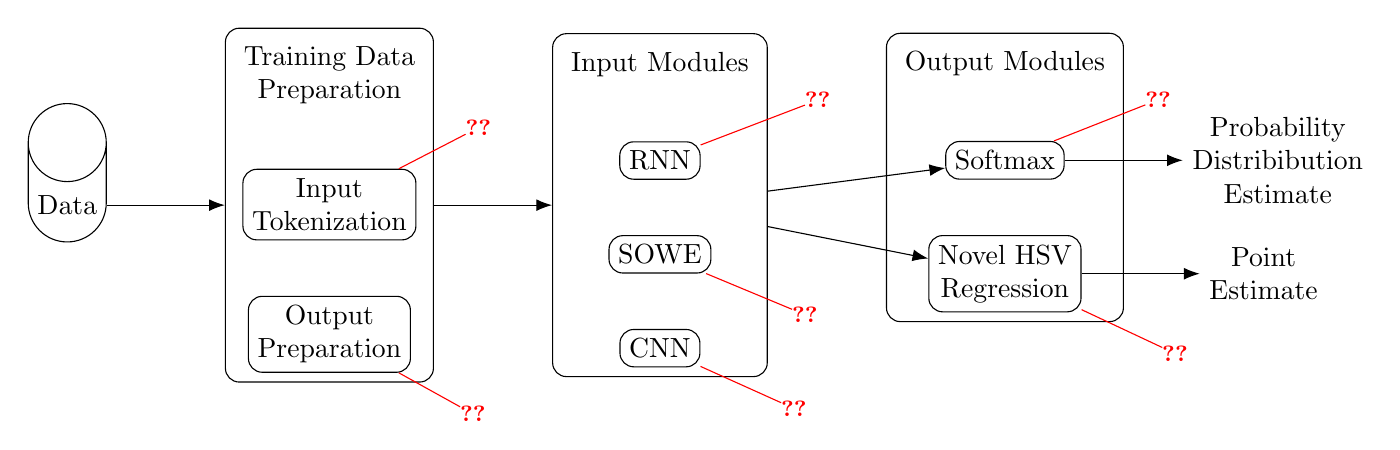
\begin{tikzpicture}
		\node (data) [cylinder, shape border rotate=90, draw, minimum height=5 em] {Data};
		
		\node (prep) [matrix, right = of data] {
			\node{Training Data \\ Preparation}; \\
			\node(inputprep)[draw]{Input\\Tokenization};\\
			\node(outputprep)[draw]{Output\\Preparation}; \\
		};
		
		\refnodeAR[xshift=-0.4cm]{sec:input-data-preparation}{inputprep};
		\refnodeBR[xshift=-0.4cm]{sec:output-data-preparation}{outputprep};
		
		\node (input) [matrix, right = of prep] {
			\node{Input Modules}; \\
			\node(rnn)[draw]{RNN}; \\
			\node(sowe)[draw]{SOWE};\\
			\node(cnn)[draw]{CNN}; \\
		};
		\refnodeBR{sec:sowemod}{sowe};
		\refnodeBR{sec:cnnmod}{cnn};
		\refnodeAR[xshift=0.3cm]{sec:rnnmod}{rnn};
		
		\node (output) [matrix, right = of input, yshift=1em] {
			\node{Output Modules}; \\
			\node(softmax)[draw]{Softmax}; \\
			\node(hsvreg)[draw]{Novel HSV \\ Regression}; \\
		};
		\refnodeAR{sec:distmod}{softmax}
		\refnodeBR{sec:point-estimation}{hsvreg}
	
	
		\node(dist)[right=of softmax]{Probability\\Distribibution\\Estimate};
		\node(point)[right=of hsvreg]{Point\\Estimate};
		
		\draw[-{Latex[length=2mm]}] (data) to (prep);
		\draw[-{Latex[length=2mm]}] (prep) to (input);
		\draw[-{Latex[length=2mm]}] (input) to (softmax);
		\draw[-{Latex[length=2mm]}] (input) to (hsvreg);
		\draw[-{Latex[length=2mm]}] (softmax) to (dist);
		\draw[-{Latex[length=2mm]}] (hsvreg) to (point);
		\end{tikzpicture}}
	\caption{The overall architecture of our systems \label{fig:arch}}
\end{figure}

\subsection{System Architecture}\label{sec:arch}
Our overall system architecture for all models is shown in \Cref{fig:arch}.
This shows how color names are transformed into distribution or point estimates over HSV color-space.

\subsection{Training Data Preparation }\label{sec:prep}
\subsubsection{Input Data Preparation}\label{sec:input-data-preparation}
We desire a color prediction model which takes as input a sequence of words that make up the colors name; rather than simply mapping from the whole phrase.
Towards this end, color names are first tokenized into individual words.
For the input into our neural network based models, those words a represented with pretrained word embeddings.

\subsubsection{Tokenization}
During tokenization a color name is split into terms with consistent spelling.
For example, \natlang{bluish kahki} would become the sequence of 3 tokens: [\natlang{blue}, \natlang{ish}, \natlang{khaki}].
Other than spelling, the tokenization results in the splitting of affixes and combine tokens.
Combining tokens and related affixes affect how multiple colors can be combined.
The full list of tokenization rules can be found in the accompanying source code.
Some further examples showing how combining tokens and affixes are used and tokenized:
\begin{itemize}
	\item \natlang{blue purple} $\mapsto$ [\natlang{blue}, \natlang{purple}].
	\item \natlang{blue-purple} $\mapsto$ [\natlang{blue}, \natlang{-}, \natlang{purple}].
	\item \natlang{bluish purple} $\mapsto$ [\natlang{blue}, \natlang{ish}, \natlang{purple}]
	\item \natlang{bluy purple} $\mapsto$ [\natlang{blue}, \natlang{y}, \natlang{purple}]
	\item \natlang{blurple} $\mapsto$ [\natlang{blue-purple}]
\end{itemize}
The final example of \natlang{blurple} is a special-case.
It is the only portmanteau in the dataset, and we do not have a clear way to tokenize it into a series of terms which occur in our pretrained embedding's vocabulary (see \Cref{sec:embeddings}).
The portmanteau \natlang{blurple} is not in common use in any training set used for creating word embeddings, so no pretrained embedding is available. \footnote{Methods do exist for generating embeddings for out of vocabulary words, particularly with FastText embeddings \parencite{bojanowski2016enriching}. But we do not investigate those here.}
As such we handle it by treating it as the single token \natlang{blue-purple} for purposes of finding an embedding.
There are many similar hyphenated tokens in the pretrained embeddings vocabulary, however (with that exception) we do not use them as it reduced the sequential modelling task to the point of being uninteresting.

\subsubsection{Embeddings}\label{sec:embeddings} 
All our neural network based solutions incorporate an embedding layer.
This embedding layer maps from tokenized words to vectors.
We make use of 300d pretrained FastText embeddings \parencite{bojanowski2016enriching}\footnote{Available from \url{https://fasttext.cc/docs/en/english-vectors.html}}.

The embeddings are not trained during the task, but are kept fixed.
As per the universal approximation theorem \parencite{leshno1993uat, SONODA2017uat} the layers above allow for arbitrary non-linear continuous transformation.
By fixing the embeddings, and learning this transformation,
we can produce estimates of colors from their embedding alone, without any training data at all, as shown in \Cref{sec:embeddingonly}.

\subsection{Output Data Preparation}\label{sec:output-data-preparation}
To train the distribution estimation models we need preprocess the training data into a distribution.
The raw training data itself, is just a collection of 
 \datapairs{} pairs -- samples from the distributions for each named-color.
This is suitable for training the point estimation models, but not for distribution estimation.
We thus convert it into a tractable form, of one histogram per output channel -- by assuming the output channels are conditionality independent of each other.


\subsubsection{Conditional Independence Assumption} \label{sec:conditional-independence-assumption}
We make the assumption that given the name of the color, the distribution of the hue, saturation and value channels are independent.
That is to say, it is assumed if the color name is known, then  knowing the value of one channel would not provide any additional information as to the value of the other two channels.
The same assumption is made, though not remarked upon, in \textcite{meomcmahanstone:color} and \textcite{mcmahan2015bayesian}.
This assumption of conditional independence allows considerable saving in computational resources.
Approximating the 3D joint distribution as the product of three 1D distributions decreases the space complexity from $O(n^3)$ to $O(n)$ in the discretized step that follows.

Superficial checks were carried out on the accuracy of this assumption.
Spearman's correlation on the training data suggests that for over three quarters of all color names, there is only weak correlation between the channels for most colors (\mbox{Q3 = 0.187}).
However, this measure underestimates correlation for values that have circular relative value, such as hue.
Of the 16 color-spaces evaluated, HSV had the lowest correlation by a large margin.
Full details, including the table of correlations, are available in supplementary materials (\Cref{sec:corrind}).
These results are suggestive, rather than solidly indicative, on the degree of correctness of the conditional independence assumption.
We consider the assumption sufficient for this investigation.

\subsubsection{Discretization} \label{sec:discretization}
For distribution estimation, our models are trained to output histograms.
This is a discretized representation of the continuous distribution.
Following standard practice interpolation-based methods can be used to handle it as a continuous distribution.
By making use of the conditional independence assumption (see \Cref{sec:conditional-independence-assumption}), we output one 256-bin histogram per channel.
We note that 24-bit color (as was used in the survey that collected the dataset) can have all information captured by a 256 bin discretization  per channel.
24 bit color allows for a total of $2^{24}$ colors to be represented, and even one-hot encoding for each of the 256 bin discretization channels allows for the same.
As such there is no meaningful loss of information when using histograms over a truely continuous estimation method, such as a Gaussian mixture model.
Although such models may have other advantages (such as the a priori information added by specifying the distribution), we do not investigating them here, instead considering the simplest non-parametric estimation model (the histogram), which has the simple implementation in a neural network using a softmax output layer.

Discretizing the data in this way is is a useful solution used in several other machine learning systems.
\textcite{oord2016pixel, DBLP:journals/corr/OordDZSVGKSK16} apply a similar discretization step and found their method to outperforming the more complex continuous distribution outputs.

For training purposes we thus convert all the observations into histograms.
One set of histograms is produced per color description present in the dataset.
We perform an uniform weight attribution of points to bins as described by \textcite{jones1984remark}. In-short, this method of tabulation is to define the bins by their midpoints, and for each point a point then probability mass is allocated the bins with midpoints to each side of the observation  in proportion to the distance.


\subsection{Color Name Representation Learning (Input Modules)}\label{sec:inputmod}
For each of the models we investigate we define an input module.
This is a portion of the over-all network which when is combined with an appropriate output module (see \Cref{sec:outputmod}) to perform either point estimation, or distribution estimation.


\subsubsection{Recurrent Neural Network(RNN)}\label{sec:rnnmod}
\begin{figure}
	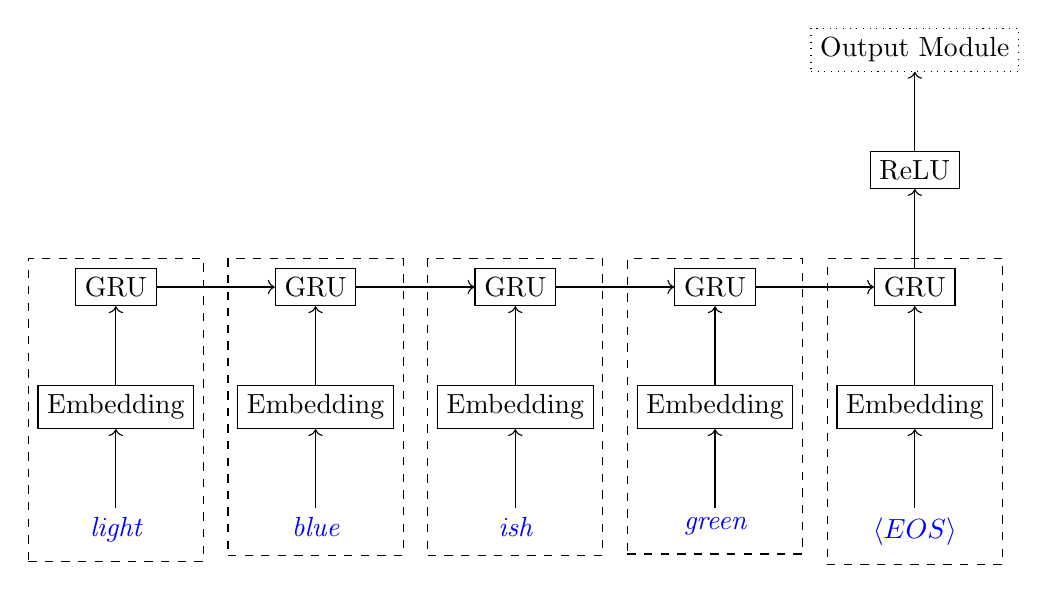
\begin{tikzpicture}
	\node (hiddenoutput)[layer] at (0,0) {ReLU};
	\node (output)[dotted, layer, above=1 of hiddenoutput] {Output Module};
	\draw[->] (hiddenoutput) to (output);
	
	\node (GRU1)[layer, below = of hiddenoutput]{GRU};
	
	\foreach[count=\i from 1] \j in {2,...,5}
	{
		\node (GRU\j)[layer, left = of GRU\i]{GRU};
		\draw[->] (GRU\j) to (GRU\i);
	}
	
	\foreach[count=\i from 1] \word in {$\langle EOS \rangle$, green, ish, blue, light}
	{
		\node (emb\i)[layer, below = of GRU\i]  {Embedding};
		\node (word\i)[word, below = of emb\i]{\word};
		\draw[->] (word\i) to  (emb\i);
		\draw[->] (emb\i) to (GRU\i);
		\node[draw,dashed,fit= (emb\i)  (word\i)  (GRU\i)] {};
	}
	
	
	\draw[->] (GRU1) to (hiddenoutput);
	\end{tikzpicture}
	
	\caption{The RNN Input module for the example input \natlang{light greenish blue}. Each dashed box represents 1 time-step. \label{fig:rnnmod}}
\end{figure}


A Recurrent Neural Network is a common choice for this kind of task,
due to the variable length of the input.
The general structure of this network, shown in \Cref{fig:rnnmod} is similar to \textcite{2016arXiv160603821M}, or indeed to most other word sequence learning models.
Each word is first transformed to an embedding representation.
This representation is trained with the rest of the network allowing per word information to be efficiently learned.
The embedding is used as the input for a Gated Recurrent Unit (GRU) 
The stream was terminated with an End of Stream (\natlang{<EOS>}) pseudo-token,
represented using a zero-vector.
The output of the last time-step is fed to a Rectified Linear Unit (ReLU).

We make use of a GRU \parencite{cho2014properties},
which we found to marginally out-perform the basic RNN in preliminary testing.
The small improvement is unsurprising, as the color names have at most 5 terms,
so longer short term memory is not required.


\subsubsection{Sum of Word Embeddings (SOWE)}\label{sec:sowemod}
Using a simple sum of word embeddings as a layer in a neural network is less typical than an RNN structure.
Though it is well established as a useful representation, and has been used an input to other classifiers such as support vector machines \parencite{White2015SentVecMeaning,novelperspective}.
Any number of word embeddings can be added to the sum, thus allowing it to handle sequences of any length.
However, it has no representation of the order.
The structure we used is shown in \Cref{fig:sowemod}.

\begin{figure}
	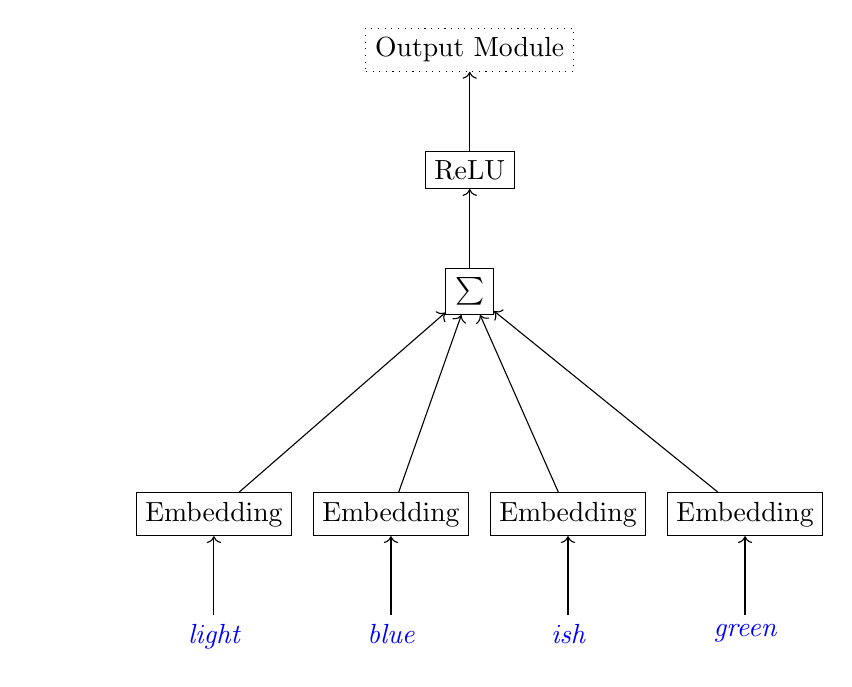
\begin{tikzpicture}
	
	\node (GRU1)[]{};
	
	\foreach[count=\i from 1] \j in {2,...,5}
	{
		\node (GRU\j)[left = 2 of GRU\i]{};
	}
	
	\node (sum)[layer, above= of GRU3, xshift=1cm]{$\sum$};
	
	\foreach[count=\i from 1] \word in {green, ish, blue, light}
	{
		\node (emb\i)[layer, below = of GRU\i]  {Embedding};
		\node (word\i)[word, below = of emb\i]{\word};
		\draw[->] (word\i) to  (emb\i);
		\draw[->] (emb\i) to (sum);
	}
	
	\node (hiddenoutput)[layer, above=of sum] {ReLU};
	\node (output)[dotted, layer, above=1 of hiddenoutput] {Output Module};
	\draw[->] (sum) to (hiddenoutput);
	\draw[->] (hiddenoutput) to (output);
	
	\end{tikzpicture}
	
	\caption{The SOWE input module for the example input \natlang{light bluish green}}
	\label{fig:sowemod}
\end{figure}



\subsubsection{Convolutional Neural Network(CNN)}\label{sec:cnnmod}
A convolutional neural network can be applied to the task by applying 2D convolution over the stacked word embeddings.
\Cref{fig:cnnmod}
We use 64 filters of size between one and the length of the longest padded embedding (5).
\pdfcomment{I can't find who first did this. Rui spoke of it.}

\begin{figure}
	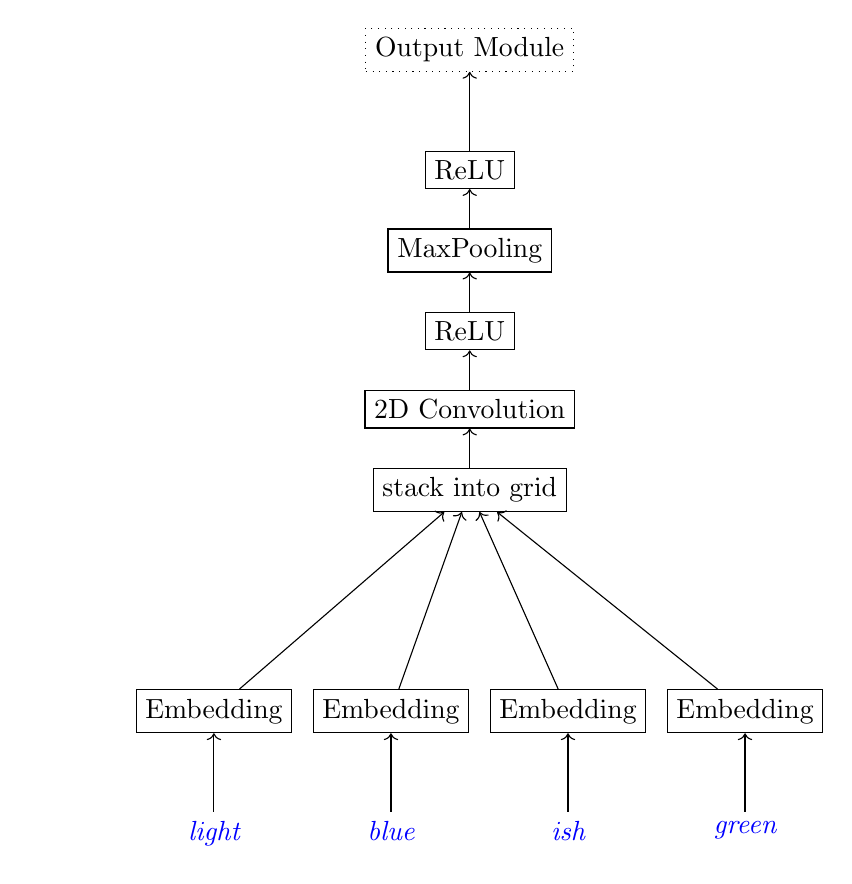
\begin{tikzpicture}
	
	\node (GRU1)[]{};
	
	\foreach[count=\i from 1] \j in {2,...,5}
	{
		\node (GRU\j)[left = 2 of GRU\i]{};
	}
	
	\node (hstack)[layer, above= of GRU3, xshift=1cm]{stack into grid};
	
	\foreach[count=\i from 1] \word in {green, ish, blue, light}
	{
		\node (emb\i)[layer, below = of GRU\i]  {Embedding};
		\node (word\i)[word, below = of emb\i]{\word};
		\draw[->] (word\i) to  (emb\i);
		\draw[->] (emb\i) to (hstack);
	}
	
	\node (conv)[layer, above= 0.5 of hstack]{2D Convolution};
	\node (innerconv)[layer, above= 0.5 of conv]{ReLU};
	\node (pool)[layer, above= 0.5 of innerconv]{MaxPooling};
	\node (hiddenoutput)[layer, above= 0.5 of pool] {ReLU};
	\node (output)[dotted, layer, above=1 of hiddenoutput] {Output Module};
	\draw[->] (hstack) to (conv);
	\draw[->] (conv) to (innerconv);
	\draw[->] (innerconv) to (pool);
	\draw[->] (pool) to (hiddenoutput);
	\draw[->] (hiddenoutput) to (output);
	
	%	\draw[->] (hstack) to (hiddenoutput);
	%	\draw[->] (hiddenoutput) to (output);
	
	\end{tikzpicture}
	
	\caption{The CNN input module for the example input \natlang{light greenish blue}}
	\label{fig:cnnmod}
\end{figure}





\subsection{Distribution and Point Estimation (Output Modules)}\label{sec:outputmod}
On top of the input module we define an output module to suit the neural network for the task fo either distribution estimation or point estimation.
The input module defines how the terms are composed into the network.
The output module defines how the network takes its hidden representation and produces an output.


\subsubsection{Distribution Estimation}\label{sec:distmod}
The distributions are trained to produce the discretized representation as discussed in \Cref{sec:discretization}.
Making use of the conditional independence assumption (see \Cref{sec:conditional-independence-assumption}), we output the three discretized distributions.
This is done using the softmax output layers, as shown in \Cref{fig:distoutmod} the three output layers.
They share a common input, but have separate weights and biases.
The loss function is given the sum of the cross-entropy for each of the three softmax outputs.


\begin{figure}
	\newcommand{\picwidth}{60pt}
	\begin{tikzpicture}
	
	\node (input)[layer, dotted]{Input Module};
	
	\node(outHue)[layer, above left = of input] {Softmax};
	\node(outSaturation)[layer, above = of input] {Softmax};
	\node(outValue)[layer, above right = of input] {Softmax};
	
	\foreach \p in {Hue, Saturation, Value} 
	{
		\draw[->] (input) to (out\p);
		
		\node(plot\p)[above = of out\p, text width=\picwidth]{
			\includegraphics[width=\picwidth]{netdia/\p}
			\\
			\p
		};
		\draw[->] (out\p) to (plot\p);
	}
	\end{tikzpicture}
	
	\caption{The Distribution Output Module \label{fig:distoutmod}}
\end{figure}


\subsubsection{Point Estimation}\label{sec:point-estimation}
Our point estimation output module is shown in \Cref{fig:pointoutmod}.
The hidden-layer from the top of the input module is feed to an four single output neurons.\footnote{Equivalently these four single neurons can be expressed as a layer with four outputs and two different activation functions.}
Two of these use the sigmoid activation function (range 0:1) to produce the outputs for the saturation and value channels.
The other two use the tanh activation function (range -1:1), they produce the intermediate output that we call $y_{shue}$ and $y_{chue}$ for the sine and cosine of the hue channel respectively.
The hue can be found as $y_{hue} =  \mathrm{atan2} \left(y_{shue}, y_{chue} \right)$.
We use the intermediate values when calculated the loss function.
During training we use the following loss function for each observation $y^\star$, and each corresponding prediction $y$.
\begin{align}
loss &= %
\frac{1}{2} \left(\sin(y^\star_{hue}) - y_{shue} \right)^2     \nonumber \\
&+ \frac{1}{2} \left(\cos(y^\star_{hue}) - y_{chue} \right)^2  \nonumber \\
&+ \left(y^\star_{sat} - y_{sat} \right)^2  \nonumber \\
&+ \left(y^\star_{val} - y_{val} \right)^2 %
\end{align}
This mean of this loss is taken over all observations in each mini-batch during training.
This loss function is continuous and correctly handles the wrap-around nature of the hue channel \parencite{WhiteRepresentingAnglesSE}.

\begin{figure}
	\newcommand{\picwidth}{60pt}
	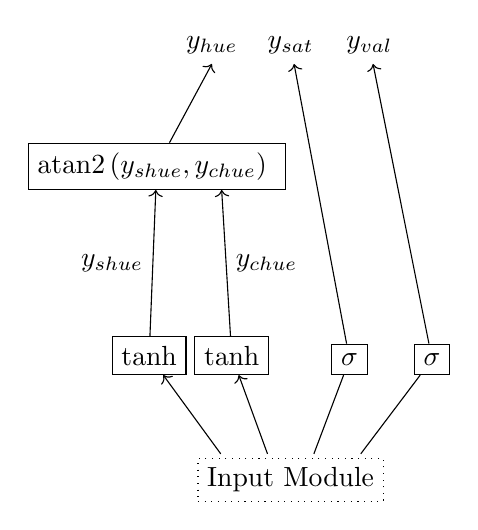
\begin{tikzpicture}
	
	\node (hiddenout)[layer, dotted]{Input Module};
	%\node (hiddenout)[above= 1 of input]{Affine with output width 4};
	%\draw[->](input) to (hiddenout);
	
	\node(outHue)[xshift=-1cm, above = 5 of hiddenout] {$y_{hue}$};
	\node(outSaturation)[above = 5 of hiddenout] {$y_{sat}$};
	\node(outValue)[xshift=1cm, above = 5 of hiddenout] {$y_{val}$};
	
	\node(Z)[above=-0.2cm of hiddenout.north]{};
	\node(Z2)[left=0cm of Z]{};%{$z_2$};
	\node(Z1)[left=0.3cm of Z2]{};%{$z_1$};
	\node(Z3)[right=0cm of Z]{};%{$z_3$};
	\node(Z4)[right=0.3cm of Z3]{};%{$z_4$};
	
	
	\node(s3)[layer, above=1 of Z3, xshift=0.5cm]{$\sigma$};
	\node(s4)[layer, above=1 of Z4, xshift=1cm]{$\sigma$};
	\draw[->](Z3) to (s3) to (outSaturation);
	\draw[->](Z4) to (s4) to (outValue);
	
	
	\node(AngHue)[layer, below = 1 of outHue, xshift=-0.7cm]{$ \mathrm{atan2} \left(y_{shue}, y_{chue} \right) $ };
	\draw[->](AngHue) to (outHue.south);
	
	\node(s1)[layer, above=1 of Z1, xshift=-1cm]{$\tanh$};
	\node(s2)[layer, above=1 of Z2, xshift=-0.5cm]{$\tanh$};
	\draw[->](Z1) to (s1);
	\draw[->](s1) to node[left]{$y_{shue}$} (AngHue);
	\draw[->](Z2) to (s2);
	\draw[->](s2) to node[right]{$y_{chue}$}  (AngHue.340);
	
	\end{tikzpicture}
	
	\caption{The Point Estimate Output Module.
		Here $\mathrm{atan2}$ is the quadrant preserving arctangent, outputting as a regularized angle (as per in all evaluations).
		\label{fig:pointoutmod}}
\end{figure}



\section{Evaluation}

\subsection{Perplexity in Color-Space}
Perplexity is a measure of how well the distribution, estimated by the model, matches reality according to the observations in the test set.
Perplexity is commonly used for evaluating language models. However here it is being used to evaluate the discretized distribution estimate.
It can loosely be thought of as to how well the model's distribution does in terms of the size of an equivalent uniform distribution.
Note that this metrics does not assume conditional independence of the color channels.

Here $\tau$ is the test-set made up of pairs consisting of a color name $t$, and color-space point $\tilde{x}$;
and  $p(\tilde{x}\mid t)$  the output of the evaluated model.
Perplexity is defined:
\begin{equation}
PP(\tau) = \exp_2{\left(
	\frac{-1}{|\tau|} 
	\sum_{
		\forall(t,(\tilde{x})) \in \tau}
	\log_2 p(\tilde{x}\mid t)\right)}
\end{equation}

As the perplexity for a high-resolution discretized model will inherently be very large and difficult to read,
we define the standardized perplexity: $\frac{PP(\tau)}{n_{res}}$,
where $n_{res}$ is the total number of bins in the discretization scheme.
For all the results we present here $n_{res} = 256^3$.
This standardized perplexity gives the easily interpretable values \emph{usually} between zero and one.
It is equivalent to comparing the relative performance of the model to that of a uniform distribution of the same total resolution.
$\frac{PP(\tau)}{n_{res}}=1$ means the result is equal what we would have to if we had distributed the probability mass uniformly into all bins in a 3D histogram.
$\frac{PP(\tau)}{n_{res}}=0.5$ means the result twice as good as if we were to simply use an uniform distribution: it is equivalent to saying that the correct bin is selected as often as it would be had an uniform distribution with half as many bins (ie larger bins with twice the area) were used.
The standardised perplexity is also invariant under different output resolutions.
Though for brevity we only  present results with 256 bins per channel, our preliminary results for using other resolutions are similar under standardized perplexity.

\pdfcomment{Should mention cross entropy and KL divergence here? Closely related to perplexity}

\subsection{Angularly Correct Calculations on HSV}\label{sec:angularly-correct}
We use the HSV color-space \parencite{smith1978color} through-out this work.
We use the format which the data is originally provided in.
In this format: hue, saturation and value all range between zero and one.
Note that hue is measured in \emph{turns}, rather than the more traditional degrees, or radians.
Having hue be measured between zero and one, like the other channels, makes the modelling task more consistent.
Were the hue to range between $0$ and $2\pi$ (radians) or between $0$ and $360$ (degrees) it would be over-weighted compared to the other channels.
This regular space means that errors on all channels can be considered equally.
Unlike many other colors spaces (CIELab, Luv etc.) the gamut is square and all values of all channels corresponds to realizable colors.


When performing calculations with the HSV color space it is important to take into account that hue is an angle.
As we are working with the color space regularized to range between zero and one for all channels,
this means a hue of one and a hue of zero are equivalent (as we measure in turns, in radian's this would be $0$ and $2\pi$).

The square error of two hue values is thus calculated as:
\begin{equation}
SE(h_1, h_2) = \min \big( \left(h_1 - h_2 \right)^2, \, \left(h_1 - h_2 -1 \right)^2  \big)
\end{equation}
This takes into account the error could be calculated clockwise or counter-clockwise.
(Note that the $-1$ term related to using units of turns, were we using radians it would be $-2\pi$)


The mean of a set of hues ($\lbrace h_1,\,\ldots,\,h_N \rbrace$) is calculated as:
\begin{equation}
\bar h = \mathrm{atan2} \Bigg(%
	\frac{1}{N} \sum_{i=1}^{i=N} \sin (h_i), \,  %
	\frac{1}{N} \sum_{i=1}^{i=N} \cos (h_i)%
\Bigg)%
\end{equation}
This gives the mean angle.
(Note again: as we measure angle in turns we use the turn trigonometric functions in implementation, though this mean is the same expression or any units).


\subsection{Evaluation Strategies}

\subsubsection{Full Task}
We make use of the  Munroe dataset as prepared by \textcite{mcmahan2015bayesian} from the results of the XKCD color survey.
The XKCD color survey \parencite{Munroe2010XKCDdataset}, collected over 3.4 million observations from over 222,500 respondents.
McMahan and Stone take a subset from Munroe's full survey, by restricting it to the responses from native English speakers, 
and removing very rare color names with less than 100 uses.
This gives a total of 2,176,417 observations and 829 color names. 
They also define a standard test, development and train split.


\subsubsection{Unseen Combinations Task} \label{sec:extrapodata}
A primary interest in using the term based models is to be able to make predictions for never before seen descriptions of colors.
For example, based on the learned understanding of \texttt{salmon} and of \texttt{bright}, from examples like \texttt{bright green} and \texttt{bright red}, we wish for the systems to make predictions about \texttt{bright salmon}, even though that description never occurs in the training data.
The ability to make predictions like this shows term-based natural language understanding.
It can't be done with the Operation Upper Bound model, which by-passes the term processing step.
%
To evaluate this generalisation capacity, we define new sub-datasets for both testing and training.
We select the rarest 100 color descriptions from the full dataset,
with the restriction that every token in a selected description must still have at least 8 uses in other descriptions in the training set.
The selected examples include multi-token descriptions such as: \texttt{bright yellow green} and also single tokens that occur more commonly as modifiers than as stand-alone descriptions such as \texttt{pale}.

The unseen combinations testing set has only observations from the full test set that do use those rare descriptions.
We define a corresponding restricted training set made up of the data from the full training set, excluding those  corresponding to the rare descriptions.
Similar is done for a restricted development set, so as no direct knowledge of the combined terms can leak during early-stopping.


By training on the restricted training set and testing on the unseen combinations, we can assess the capacity of the models to make predictions for color descriptions not seen in training.
A similar approach was used in \textcite{acl2018WinnLighter} and in \textcite{DBLP:journals/corr/AtzmonBKGC16}.
We contrast this to the same models when trained on the full training set to see how much accuracy was lost.


\subsubsection{Order Task}
It is believed that the order of words in a color description to matters, at least to some extent.
For example, \natlang{greenish brown} and \natlang{brownish green} are distinct, if similar, colors.
To assess the models on their ability to make predictions when order matters we construct the order test set.
This is a subset of the full test set containing only descriptions with terms that occur in multiple different orders.
There are 76 such descriptions in the full dataset.
Each of which has exactly one alternate ordering.
This is unsurprising as while color descriptions may have more than 2 terms, normally one or more of the terms is a joining token such as \natlang{ish} or \natlang{-}.
We only constructed a order testing set, and not a corresponding training set, as this is an evaluation using the model trained on the full training data.



\subsection{Operational Upper-bounds}
To establish an rough upper-limit on the modelling results we evaluate a direct method which bypasses the language understanding component of the task.
These direct methods do not process term-by-term, they do not work with the language at all.
They simply map from the exact input text (no tokenization) to the pre-calculated distribution or mean of the training data for the exact color name.
This operational upper bounds bypass the compositional language understanding part of the process.
It is as if the input module (as discussed in \Cref{sec:inputmod}) perfectly resolved the sequence of terms into a single item.


They represent an approximate upper bound, as they fully exploit all information in the training data for each input.
There is no attempting to determine how each term affects the result.
We say approximate upper-bound, as it is not strictly impossible that the term-based methods may happen to model the test data better than can be directly determined by training data as processed per exact color name.
This would require learning how the terms in the color name combine in a way that exceeds the information directly present in the training data per class.
It is this capacity of learning how the terms combine that allow for the models to predict the outputs for combinations of terms that never occur in the training data (\Cref{sec:extrapodata}).
Doing this in a way that generalizes to get better results than the direct exploitation of the training data, would require very well calibrated control of (over/under)-fitting.


\subsubsection{Operational Upper-bound for Distribution Estimation: KDE}\label{sec:direct-histogram} \label{sec:kernel-density-based-smoothing}
To determine an operational upper-bound for the distribution estimation tasks,
we use kernel-density estimation (KDE) in a formulation for non-parametric estimation \parencite{silverman1986density}.
The KDE effectively produces a smoothed histogram.
It caused adjacent bins to have most similar probabilities, thus matching to the mathematical notion of a continuous random variable.
This is applied on-top of the histogram used for the training data.
We use the Fast Fourier Transform (FFT) based KDE method of the \textcite{silverman1982algorithm}.
We use a Gaussian kernel, and select the bandwidth per color description based on leave-one-out cross validation on the training data.
A known issue with the FFT-based KDE method is that it has a wrap-around effect near the boundaries where mass that would be assigned outside the boundaries is instead assigned to the bin on the other side.
For the value and saturation channels we follow the standard solution of initially defining additional bins outside the true boundaries, then discard those bins and rescale the probability to one.
For the hue channel this wrap-around effect is exactly as desired.

In our evaluations using KDE rather than just the training histograms directly proved much more successful on all distribution estimation tasks.
This is because it avoids empty bins, and effectually interpolates probabilities between observations.
Thus improving the results
We found in preliminary investigations that using KDE based method to be much better than add-one smoothing.

We also investigated applying the KDE to the training data,  before training our term-based neural network based distribution models.
Results for this can be found in \Cref{sec:smoothed-results}.
In brief, we found that smoothing the training data does not significantly effect the result of the neural network based models.
As discussed in \Cref{sec:quantitative-results}, this is because the neural networks are able to learn the smoothness relationship of adjacent bins.


Our KDE based operational upper bound for distribution estimation bypassed the natural language understanding part of the task,
and directly uses the standard non-parametric probability estimation method to focus solely on modelling the distributions.
Matching its performance indicates that a model is effectively succeeding well at both the natural language understanding component and the distribution estimation component.


\subsubsection{Operational Upper-bound for Point Estimation: Mean-point}
In a similar approach, we also a method that directly produces a point estimate from a color name.
We define this by taking the mean of all the training observations for a given exact color name.
The mean is taken in the angularly correct way (as discussed in \Cref{sec:angularly-correct}).
Taking the mean of all the observations give the theoretically optimal solution to minimizing the squared error on the training data set.
As with our direct distribution estimation method, this bypasses the term based language understanding, and directly exploits the training data.
It thus represents an approximate upper bound on the point estimation performance of the term based models.
Though as discussed in \Cref{sec:intro}, the notion of mean and of minimizing the square error is not necessarily the correct way to characterize selecting the optimal point estimate for colors.
It is however a consistent way to do so, and so we use it for our evaluations.



\section{Experimental Setup}

\subsection{Implementation}
The implementation of the all models was in the Julia programming language \parencite{Julia}.
The full implementation is included in the supplementary materials.
can be downloaded from the GitHub repository.\footnote{Implementation source is at \url{https://github.com/oxinabox/ColoringNames.jl}}
The machine learning components make heavy use of the MLDataUtils.jl\footnote{MLDataUtils.jl is available from \url{https://github.com/JuliaML/MLDataUtils.jl}} and TensorFlow.jl,\footnote{TensorFlow.jl is available from \url{https://github.com/malmaud/TensorFlow.jl}} packages.
The latter of which we enhanced significantly to allow for this work to be carried out.
The discretization and the KDE for the Operational Upper Bound is done using KernalDensityEstimation.jl.%
\footnote{KernalDensityEstimation.jl  is available from \url{https://github.com/JuliaStats/KernelDensity.jl}}


\subsection{Common Network Features}
Drop-out\parencite{srivastava2014dropout}  is used on all layers, other than the embedding layer, with threshold of 0.5 during training.
The network is optimized using Adam \parencite{kingma2014adam}, using a learning rate of 0.001.
Early stopping is checked every 10 epochs using the development dataset.
Distribution estimation methods are trained using full batch (where each observation is a distribution) for every epoch.
Point Estimation trains using randomized mini-batches of size $2^{16}$ observations (which are each color-space triples).
All hidden-layers, except as otherwise precluded (in side the convolution, and in the penultimate layer of the point estimation networks) have the same width 300, as does the embedding layer.



\section{Results}


\documentclass[11pt,a4paper]{article}
%\usepackage[author={Lyndon}]{pdfcomment}

\usepackage{booktabs}
\usepackage{tikz}
\usepackage{graphicx}
\usepackage[space]{grffile}


\begin{document}
\clearpage


\def\maincolors{%
	brown-orange,
	orange-brown,	
	yellow-orange,
	orange-yellow,
	brownish green,
	greenish brown,
	bluish grey,
	greyish blue,
	pink-purple,
	purple-pink,
	green,
	greenish,
	purple,	
	purplish,
	brown,
	brownish,
	black,
	white,
	grey%
}

\def\oovcolors{
	%	brownish 1Green,
	%	bluish gray,
	1Brown,
	1Green,
	1Purple,
	gray,
	1Gray%
}


\tikzset{lastline/.style={opacity=1}};
\newcommand{\distfigs}[2]{
	\begin{tikzpicture}%
	\foreach[count=\mdlii from 0] \mdlname in #1 {%
		\node at (3.1*\mdlii cm, -1cm) {\sffamily \mdlname};%
		\foreach[count=\colii from 0] \colorname in #2 {%
			\xdef\topy{1.1*\colii}
			\node at (3.1*\mdlii cm, \topy cm) %
			{\includegraphics[height=0.95cm]{%
					figs/demo/dist/\mdlname/\colorname}%
			};%

		}%
		\xdef\topy{\topy+1}
		\node at (3.1*\mdlii cm, -1cm) {\sffamily \mdlname};%
		\node at (3.1*\mdlii cm, \topy) {\sffamily \mdlname};%
	}%
	%

	\draw[dashed] (1.555, -1.1) -- (1.555, \topy);%
	\draw[lastline] (3*1.555,-1.1) -- (3*1.555, \topy);%
	\draw[dashed,lastline] (5*1.555,-1.1) -- (5*1.555, \topy);%
	%
	\end{tikzpicture}%
}%

\subsection{Quantitative Results}

\newcommand{\pointfigs}[3]{
	\begin{tikzpicture}%
	\foreach[count=\mdlii from 0] \mdlname in #1 {%
		
		\node(fig\mdlname) at (3.1*\mdlii cm, 0) %
		{\includegraphics[height=#3 cm]{%
				figs/demo/point/\mdlname/#2}%
		};%
		\node[below = -0.7 of fig\mdlname] {\sffamily \mdlname};%
		\node[above = -0.7 of fig\mdlname] {\sffamily \mdlname};%
	}%
	\end{tikzpicture}%
}%


\begin{figure}
	\distfigs{{Direct, Direct-smoothed, SOWE, SOWE-smoothed}}{\maincolors}
	\caption{Some examples of the output distribution estimations from the models trained on the full dataset} \label{fig:distout1}
\end{figure}

\begin{figure}
	\distfigs{{CNN, CNN-smoothed, RNN, RNN-smoothed}}{\maincolors}
	\caption{Some examples of the output distribution estimations from the models trained on the full dataset} \label{fig:distout2}
\end{figure}

\begin{figure}
	\pointfigs{{Direct, SOWE, CNN, RNN}}{maincolors}{18}
	\caption{Some examples of the output distribution estimations from the models trained on the full dataset} \label{fig:pointout}
\end{figure}

\Cref{fig:distout1} and \Cref{fig:distout2} show some examples of distribution estimates for the models trained on the full data sets.
\Cref{fig:pointout} shows similar examples for point estimates.
It can be seen the the model's outputs using term based estimations are generally similar to the direct outputs, as is intended.
This aligns with the strong results found in that quantitative evaluations in \Cref{sec:quantitative-results}.
The models are correctly fitting to estimate the colors.

When considering the pairs of outputs that differ only in word order, such as \natlang{purple-pink} and \natlang{pink-purple} the models differ in behaviour.
The Direct results show that the ground truth is that such color name pairs are subtly different but very similar.
The SOWE models is unable to take into account word order at all, and so produces identical output for both.
The CNN models produce very similar outputs but not strictly identical -- spotting the different requires very close observation.
This is in-line with the different filter sizes allowing it to to use n-gram features, and it finding the unigram features most useful.
The RNN produces the most strikingly different results.
It seems the first term dominates the final output: \natlang{purple-pink} is more purple, and  \natlang{pink-purple} is more pink.
We can see that the first time is not solely responsible for the final output however, as \natlang{purple-pink}, \natlang{purple} and \natlang{purplish} (tokenized as \natlang{purple}, \natlang{ish}) are all different.
It is surprising that the RNN is dominated by the first term and not the latter terms\footnote{So much so that we double checked out implementation to be sure it wasn't processing the inputs backwards.} this shows the GRU is functioning to remember the earlier inputs.
This is happening too strongly however, as it causes the colors to differ to much.


The effect of the models on the smoothness when estimating distributions is interesting.
As expected, applying the KDE based smoothing to the training data produces a smoother output.
Further: the all the outputs of the neural network models are smoother than the correspond direct models.
This is true both when trained on smoothed and on unsmoothed training data.
The models are learning that adjacent bins should have similar output values, as this is a common feature of all the training data no matter the color.
An effect of this is that while the models capture the highly asymmetrical shapes of most distributions well,
they do not do well at capturing small dips.
Larger multi-modes as seen in the achromatic colors like \natlang{white}, \natlang{grey}, \natlang{black}, \natlang{white}, are captured; but smaller dips such as the hue of \natlang{greenish} being mostlikely to be either side of the green spectrum are largely filled in.
In general, it seems clear that the smoothing of the training data is not required for the neural network based models.




%%%%%%%%%%%%%%%%%%%%%%%%%%%%%%%%%%%%%%%%%%%%%%%%%%%%%%%%%%%





\subsection{Completely Unseen Color Estimation From Embedding Only}\label{sec:embeddingonly}
\Cref{fig:oovdist} and \Cref{fig:oovpoint} show quantitative examples of estimated colors for color-names that do not occur in the training data (or testing) at all.
This is even more extreme than the extrapolation tasks considered in \Cref{tbl:distextrapo} and \Cref{tbl:pointextrapo} where the terms appeared in training but not the combination of terms.
In these examples the terms are never occurred in the training data, but out models exploit the fact that they work by transforming the embedding space to use the word embeddings to predict the colors for them anyway.
There is no equivalent for this in the direct models.
While \natlang{Grey} and \natlang{gray} never occur in the training data; \natlang{grey} does, and it is near by in embedding space; similar is true for the other colors that vary by capitalization.
We only present a few examples of single term colors here, and no quantitative investigation, as this is merely a matter of interest.

It is particularly interesting to note that that all the models both for point estimation and distribution estimation make similar estimations for each color.
They do well on the same colors and make similar mistakes on the colors they do poorly at.
The saturation of \natlang{Gray} is estimated too high, making it appear too blue/purple, this is also true of \natlang{grey} though to a much lesser extent.
\natlang{Purple} and \natlang{Green} produce generally reasonable estimates.
The hue for \natlang{Brown} is estimated as having too much variance, allowing the color to swing into the red or yellowish-green parts of the spectrum.
In general the overall quality of each model seems to be in line with that found in the quantitative results for the full tests.







\begin{figure}
	\distfigs{{SOWE, SOWE-smoothed,CNN, CNN-smoothed}}{\oovcolors}
	\tikzset{lastline/.style={opacity=0}}
	\distfigs{{RNN, RNN-smoothed}}{\oovcolors}
	\tikzset{lastline/.style={opacity=1}}
	
	\caption{Some example distribution estimations for colors names which are completely outside the training data. The terms: \natlang{Brown}, \natlang{gray}, \natlang{Gray}, \natlang{Green}, and \natlang{Purple}, do not occur in any of the color data; however \natlang{brown}, \natlang{grey} \natlang{green}, and \natlang{purple} do occur.} \label{fig:oovdist}
\end{figure}

\begin{figure}
\pointfigs{{SOWE, CNN, RNN}}{oovcolors}{5}
\caption{Some example point estimates for colors names which are completely outside the training data. The terms: \natlang{Brown}, \natlang{gray}, \natlang{Gray}, \natlang{Green}, and \natlang{Purple}, do not occur in any of the color data; however \natlang{brown}, \natlang{grey} \natlang{green}, and \natlang{purple} do occur.} \label{fig:oovpoint}
\end{figure}

\end{document}
\documentclass[11pt,a4paper]{article}
\usepackage[author={Lyndon}]{pdfcomment}

\usepackage{booktabs}

\usepackage{booktabs}
\usepackage{pgfplotstable}
\usepackage{pgfplots}
\pgfplotsset{compat=1.14}


\DeclareMathVersion{tabularbold}
\SetSymbolFont{operators}{tabularbold}{OT1}{cmr}{b}{n}


% Center all floats
\makeatletter
\g@addto@macro\@floatboxreset{\centering}
\makeatother

\usepackage{cleveref}

\newcommand{\empmodel}{Non-compositional baseline} 
\begin{document}
	



\pgfkeys{
	/pgf/number format/.cd, fixed, precision=3, fixed zerofill=true
}

\pgfplotstableset{
	col sep=comma,
	header=has colnames,
	column type={c},
	ignore chars={"},
	clear infinite,
	empty cells with={--},
	every head row/.style={before row=\toprule,	after row=\midrule},
	columns/method/.style={
		reset styles,
		string type,
		column name=Method,
		string replace*={Operational Upper Bound}{Non-compositional Baseline}},
	%
	boldcell/.style = {
		postproc cell content/.append style={
			@cell content/.add={\mathversion{tabularbold}}{}
		}
	},
	%
	greycell/.style = {
		postproc cell content/.append style={
			@cell content/.add={\color{gray}}{}
		}		
	}
}
\pgfplotstableset{distresults/.append style={%
		columns={method, perpstd},
		columns/perp/.style={column name=$PP$},
		create on use/perpstd/.style={
			create col/expr={\thisrow{perp}/(256*256*256)},
		},
		columns/perpstd/.style={column name=$\frac{PP}{256^3}$},
		%
		every row 0 column 1/.style={greycell}
	},%
	%%%%%%%%%%%%%%%%%%%%%%%%%%%%%%%%%%%%%%%%%%%%%%%%
	extrapodistresults/.append style={
		every row 0 column 1/.style={greycell},
		every row 0 column 2/.style={greycell},
		%
		columns={method, nxperpstd, xperpstd},
		columns/nxperpstd/.style={column name={\shortstack{\small Full\\Training Set\\$\frac{PP}{256^3}$}}},
		columns/xperpstd/.style={column name={\shortstack{\small Restricted\\Training Set\\$\frac{PP}{256^3}$}}},
		%		
		create on use/xperpstd/.style={
			create col/expr={\thisrow{extrapolatingperp}/(256*256*256)},
		},
		create on use/nxperpstd/.style={
			create col/expr={\thisrow{nonextrapolatingperp}/(256*256*256)},
		},
	}
}


\pgfplotstableset{pointresults/.append style={%
		columns={method,mse},
		columns/mse/.style={column name={$MSE$}},
		%
		every row 0 column 1/.style={greycell},
		every row 4 column 1/.style={greycell},
	},%
	extrapopointresults/.append style={
		columns={method, nonextrapolatingmse, extrapolatingmse},
		columns/nonextrapolatingmse/.style={column name=\shortstack{\small Full\\Training Set\\$MSE$}},
		columns/extrapolatingmse/.style={column name=\shortstack{\small Restricted\\Training Set\\$MSE$}},
		%		
		every row 0 column 1/.style={greycell},
		every row 4 column 1/.style={greycell},
		every row 0 column 2/.style={greycell},
		every row 4 column 2/.style={greycell},
	},
}
	

\subsection{Quantitative Results}\label{sec:quantitative-results}

Overall, we see that our models are able to learn to estimate colors based on sequences of terms.
From the consideration of all the results shown in \Cref{tbl:pointfull,tbl:distfull,tbl:distord,tbl:pointord,tbl:pointextrapo,tbl:distextrapo}, 
the CNN and SOWE models perform almost as well as the \empmodel{}.
With the SOWE having a marginal lead for distribution estimation,
and the CNN and SOWE being nearly exactly equal for most point estimation tasks.
We believe the reason for this is that the SOWE is an easier to learn model from a gradient descent perspective:
it is a shallow model with only one true hidden layer.
The RNN did not perform as well at these tasks.
While it is only marginally behind the SOWE and CNN on the full point estimation task (\Cref{tbl:pointfull}), on all other tasks for both point estimation and distribution estimation it is significantly worse.
This may indicate that it is hard to capture the significant relationships between terms in the sequence.
However, as shown \Cref{sec:quantitative-results} it did learn generally acceptable colors, but it is not as close a match to the population's expectation.


%%%%%%%%%% Full

\begin{table}
	\caption{\label{tbl:distfull} The results for the \textbf{full distribution estimation task}. Lower perplexity (PP) is better.}
	%	\resizebox{\columnwidth}{!}{
	\pgfplotstabletypeset[distresults,
	every row 1 column 1/.style={boldcell},
	]{results/regular/res_dist_full.csv}
	%	}
\end{table}



\begin{table}
	\caption{\label{tbl:pointfull} The results for the \textbf{full point estimation task}. Lower mean squared error (MSE) is better.}
	%	\resizebox{\columnwidth}{!}{
	\pgfplotstabletypeset[pointresults,
	every row 2 column 1/.style={boldcell},
	every row 1 column 1/.style={boldcell}
	]{results/regular/res_point_comb_full.csv}
	%	}
\end{table}

\subsubsection{Ordered Task}
The performance of SOWE on the order tasks (\Cref{tbl:distord,tbl:pointord}) is surprising.
For the distribution estimation it outperforms the CNN, and for point estimation it ties with the CNN.
The CNN and RNN, can take into account word order, but the SOWE model cannot.
The good results for SOWE suggest that the word-order is not very significant for color names.
While word order matters, different colors with the same terms in different order are similar enough that it still performs very well.
In theory the models that are capable of using word order have the capacity to ignore it, and thus could achieve a similar result.
An RNN can learn to perform a sum of its inputs (the word embeddings),
and the CNN can learn to weight all non-unigram filters to zero.
In practice we see that for the RNN in particular this clearly did not occur.
This can be attributed to the more complex networks being more challenging to train via gradient descent.
It seems that color-naming is not a task where word order substantially matters,
and thus the simpler SOWE model excels.



%%%%%%% ORDER

\begin{table}
	\caption{\label{tbl:distord} The results for the \textbf{order distribution estimation task}. Lower perplexity (PP) is better. This is a subset of the full test set containing only tests where the order of the words matters.}
	%	\resizebox{\columnwidth}{!}{
	\pgfplotstabletypeset[distresults,
	every row 1 column 1/.style={boldcell},
	]{results/regular/res_dist_ord.csv}
	%	}
\end{table}


\begin{table}
	\caption{\label{tbl:pointord} The results for the \textbf{order point estimation task}. Lower mean squared error (MSE) is better. This is a subset of the full test set containing only tests where the order of the words matters.}
	%	\resizebox{\columnwidth}{!}{
	\pgfplotstabletypeset[pointresults,
	every row 1 column 1/.style={boldcell},
	every row 2 column 1/.style={boldcell},
	%3
	%4
	%
	every row 5 column 1/.style={boldcell},
	every row 6 column 1/.style={boldcell}
	]{results/regular/res_point_comb_ord.csv}
	%	}
\end{table}


\subsubsection{Unseen Combinations of Terms}
The SOWE and CNN models are able to generalize well to making estimates for combinations of color terms that are not seen in training.
\Cref{tbl:distextrapo,tbl:pointextrapo} show the results of the model on the test set made up of rare combinations of color names (as described in \Cref{sec:extrapodata}) for the restricted training set (which does not contain those terms).
These results on this test set are compared with the same models when trained on the full training set.
The Operation Upper Bound models are unable to produce estimates from the unseen combinations testing set as they do not process the color names term-wise.
The RNN models continue to perform badly on the unseen combination of terms task for both point and distribution estimation.

On distribution estimation (\Cref{tbl:distextrapo}) the SOWE results are only marginally worse for the restricted training set as they are for the full training set.
The CNN results are worse again, but they are still better than the results on the full test-set.
The distribution estimates are good on absolute terms, having low evaluated perplexity.

In the point estimation task (\Cref{tbl:pointextrapo}) the order is flipped with the CNN outperforming the SOWE model.
In-fact the CNN actually performs better with the restricted training set.
This may be due to the CNN not fitting to the training data as well as the SOWE,
as on the full training set (for this test set) we see the SOWE outperforms the CNN.
This suggests that the CNN point estimation model may be better at capturing the shared information about term usages, at the expense of fitting to the final point.
%\pdfcomment{Does this make sense?}
Unlike for distribution estimates, the unseen color point estimates are worse than the overall results from the full task (\Cref{tbl:pointfull}), though the errors are still small on an absolute scale.



%%%%%%%% Extrapo


\begin{table}
	\caption{\label{tbl:distextrapo} The results for the \textbf{unseen combinations distribution estimation task}. Lower perplexity (PP) is better. This uses the unseen test set: a subset of the full test set contain only rare word combinations. In the restricted training set results these rare word combinations were removed from the training and development sets. In the full training set results the whole training and development stet was used, including the rare words that occur in the test set.}
	%	\resizebox{\columnwidth}{!}{
	\pgfplotstabletypeset[extrapodistresults,
	every row 1 column 1/.style={boldcell},
	every row 1 column 2/.style={boldcell}
	]{results/regular/res_dist_extrapo.csv}
	%	}
\end{table}


\begin{table}
	\caption{\label{tbl:pointextrapo} The results for the \textbf{unseen combinations point estimation task}. Lower mean squared error (MSE) is better. This uses the unseen test set: a subset of the full test set contain only rare word combinations. In the restricted training set results these rare word combinations were removed from the training and development sets. In the full training set results the whole training and development stet was used, including the rare words that occur in the test set.}
	%	\resizebox{\columnwidth}{!}{
	\pgfplotstabletypeset[extrapopointresults,
	every row 1 column 1/.style={boldcell},
	every row 2 column 2/.style={boldcell},
	]{results/regular/res_point_comb_extrapo.csv}
	%	}
\end{table}

\subsubsection{Extracting the mean from the distribution estimates}

In the point estimation results discussed so far have been from models trained specifically for point estimation (as described by \Cref{sec:point-estimation}).
However, it is also possible to derive the mean from the distribution estimation models.
Those results are also presented in \Cref{tbl:pointfull,tbl:pointord,tbl:pointextrapo}.
In general these results perform marginally worse (using the MSE metric) than their corresponding modules using the point estimation output module.
We note that for the \empmodel{}, the distributions mean is almost identical to the true mean of points, as expected.

Beyond the output module there are a few key differences between the point estimation modules and the distribution estimate modules.
When training distribution estimation models, all examples of a particular color name is grouped into a single high information training observation using the histogram as the output.
Whereas when training for point estimation, each example is processed individually (using minibatches).
This means that the distribution estimating models fit to all color names with equal priority. % \pdfcomment{Can a good analogy to microaveraging and macroaveraging be made?}.
Whereas for point estimates, more frequently used color names have more examples, and so more frequent color names are fit with priority over rarer ones.
Another consequence of using training per example using random minibatches, rather than aggregating and training with full batch, is increased resilience to to local minima \parencite{lecun2012efficient}.
One of the upsides of the aggregated training used in distribution estimation is that it trains much faster as only a small number of high-information training examples are processed, rather than a much larger number of individual observations.
It may be interesting in future work to consider training the distribution estimates per example using one-hot output representations; thus making the process similar to that used in the point estimate training.
We suspect that such a method may have trouble learning the smoothness of the output space (as discussed in \Cref{sec:learnedsmoothness}).


\subsection{Training set results}

To investigate our supposition that the SOWE, is a much easier function to fit via gradient descent, as compared to RNN, or CNN, we consider the error rate on the fuill training set during the training of the models.
These plots are shown in \Cref{fig:disttrainloss,fig:pointtrainloss}.
These plots seem to support the supposition, as the SOWE training error decreases notably faster (it is a steaper curve) in both cases.
This corresponds to a easier error surface in network parameter (weights and biases) space, with less points of low gradient, or near local minima.
If we compare the final loss of each method on the training set, before it was stopped due to early stopping against the test set results in  \Cref{tbl:distfull,tbl:pointfull}
we find they are similar,  particularly for distribution estimation ( \Cref{tbl:distfull,fig:disttrainloss}).
While for for point estimation (\Cref{fig:pointtrainloss,tbl:pointfull}), on the testset CNN and SOWE perform similarly, but RNN performs much worse, while in training the performance of CNN is roughly midway between SOWE and RNN.
In all cases, the absolute error in training has become small relative the to the natural variation in the training set (as perfect fit is not possible as the training data varies).
\todo{add the noncompositional model to the training plots?}
With further model tweaking, to increase the representative capacity while regularizing against overfitting more performance may be achieved on some or all models.
\todo{Say more here?}


%%%%%%%%%%%%%%%%%%%%%%%%%%%%%%%%%%%%%%%%%%%%%%%%%%%%%%%%%%%%%%%%%%%%%%%%%%%%%%%%%%%%%%%%%%%%%%%%%%%%%%%%%%%
% Training set loss plots


\pgfplotsset{
	trainingloss/.style={
		xlabel = {Epoch},
		mark = x,
 		y tick label style={
			/pgf/number format/.cd,
			fixed,
			fixed zerofill,
			precision=3,
			/tikz/.cd
		},
		x tick label style={
			/pgf/number format/.cd,
			fixed,
			precision=0,
			/tikz/.cd
		},
	},
}

\begin{figure}
	\begin{minipage}{0.7\textwidth}
		\begin{tikzpicture}
			\begin{axis}[
			trainingloss,
			title={Distribution Estimators, Training Error},
			ylabel={$\frac{PP}{256^3}$},
			]
			\addplot table [y=SOWE-STDPERP, x=Step, col sep=comma] {results/training/distest-perplexity.csv};
			\addplot table [y=CNN-STDPERP, x=Step, col sep=comma] {results/training/distest-perplexity.csv};
			\addplot table [y=RNN-STDPERP, x=Step, col sep=comma] {results/training/distest-perplexity.csv};
			\legend{{SOWE},{CNN},{RNN}};
			\end{axis}
		\end{tikzpicture}
	\end{minipage}
	\hspace{0.5cm}
	\begin{minipage}{0.2\textwidth}
	Final Training Performance\\
	\pgfplotstabletypeset[columns/res/.style={column name=$\frac{PP}{256^3}$}]{
		method, res
		SOWE, 0.0571749749549454
		CNN, 0.0699227578631911
		RNN, 0.080777487788597
	}
	\end{minipage}
	\caption{The training set error of the distribution estimation models, when trained on the full dataset. Note that the plots stop when the model ceased training due to the development set error rising (early stopping). \label{fig:disttrainloss}}.
\end{figure}


\begin{figure}
	\begin{minipage}{0.7\textwidth}
		\begin{tikzpicture}
		\begin{axis}[
			trainingloss,
			title={Point Estimators, Training Error},
			ylabel={MSE},
			scaled y ticks={real:3}, % divide by 3 to make mean (raw data is sum)
			ytick scale label code/.code={},
			]
			\addplot table [y=SOWE, x=Step, col sep=comma] {results/training/pointest.csv};
			\addplot table [y=CNN, x=Step, col sep=comma] {results/training/pointest.csv};
			\addplot table [y=RNN, x=Step, col sep=comma] {results/training/pointest.csv};
			\legend{{SOWE},{CNN},{RNN}};
		\end{axis}
		\end{tikzpicture}
	\end{minipage}
	\hspace{0.5cm}
	\begin{minipage}{0.2\textwidth}
		Final Training Performance\\
	\pgfplotstabletypeset{
		method, MSE
		SOWE, 0.13222543895244598	
		CNN, 0.13548657298088074
		RNN, 0.14894478023052216
	}
	\end{minipage}

	\caption{The training set error of the point estimation models, when trained on the full dataset. Note that the plots stop when the model ceased training due to the development set error rising (early stopping). \label{fig:poin ttrainloss}}
\end{figure}




\end{document}


\subsection{Completely Unseen Color Estimation From Embedding Only}\label{sec:embeddingonly}
As an interesting demonstration of how the models function by learning the transformation from the embedding space to the output we briefly considers the outputs for color-names that do not occur in the training data (or testing) at all.
This is even more extreme than the unseen combinations task considered in \Cref{tbl:distextrapo} and \Cref{tbl:pointextrapo} where the terms appeared in training, but not the combination of terms.
In the examples shown in \Cref{fig:oovdist} and \Cref{fig:oovpoint}, the terms never occurred in the training data at all, but out models exploit the fact that they work by transforming the word-embedding space to predict the colors.
There is no equivalent for this in the direct models.
While \natlang{Grey} and \natlang{gray} never occur in the training data; \natlang{grey} does, and it is near-by in word-embedding space.
Similar is true for the other colors that vary by capitalization.
We only present a few examples of single term colors here, and no quantitative investigation, as this is merely a matter of interest.

It is particularly interesting to note that that all the models make similar estimations for each color.
This occurs both for point estimation and for distribution estimation.
They do well on the same colors and make similar mistakes on the colors they do poorly at.
The saturation of \natlang{Gray} is estimated too high, making it appear too blue/purple, this is also true of \natlang{grey} though to a much lesser extent.
\natlang{Purple} and \natlang{Green} produce generally reasonable estimates.
The hue for \natlang{Brown} is estimated as having too much variance, allowing the color to swing into the red or yellowish-green parts of the spectrum.
This suggests that in general all models are learning a more generally similar transformation of the space.
In general the overall quality of each model seems to be in line with that found in the results for the full tests.


\begin{figure}
	\distfigs{{SOWE/SOWE, CNN/CNN, RNN/RNN}}{\oovcolors}	
	\caption{Some example distribution estimations for colors names which are completely outside the training data. The terms: \natlang{Brown}, \natlang{gray}, \natlang{Gray}, \natlang{Green}, and \natlang{Purple}, do not occur in any of the color data; however \natlang{brown}, \natlang{grey} \natlang{green}, and \natlang{purple} do occur.} \label{fig:oovdist}
\end{figure}

\begin{figure}
	\pointfigs{{SOWE/SOWE, CNN/CNN, RNN/RNN}}{oovcolors}{5}
	\caption{Some example point estimates for colors names which are completely outside the training data. The terms: \natlang{Brown}, \natlang{gray}, \natlang{Gray}, \natlang{Green}, and \natlang{Purple}, do not occur in any of the color data; however \natlang{brown}, \natlang{grey} \natlang{green}, and \natlang{purple} do occur.} \label{fig:oovpoint}
\end{figure}



\section{Conclusion}
We have presented three input modules (SOWE, CNN, RNN),
and two output modules (distribution estimate, and point estimate)
suitable for using machine learning to make estimates about color based on the terms making up its name.
We contrasted these to a practical Operational Upper Bound model for each task which bypassed the term-wise natural language understanding component of the problem.
We found the results for SOWE, and CNN were very strong, approaching this upper bound.


A key take away from our results is that using a SOWE should be preferred over an RNN for short phrase natural language understanding tasks when order is not a very significant factor.
The RNN is the standard type of model for this task.
However, we find its performance to be significantly exceeded by the SOWE and CNN.
The SOWE is an unordered model correspondent to a bag of words.
The CNN over word embeddings is correspondent to a bag of ngrams, in our case as bag of all 1,2,3,4 and 5-grams.
This means the CNN can readily take advantage of both fully ordered information, using the filters of length 5, down to unordered information using the filters of length one.
The RNN however must fully process the ordered nature of its inputs, as its output comes only from the final node.
It would be interesting to further contrast a bidirectional RNN.

In a broader context, we envisage the distribution learned for a color name can be used as a prior probability and when combining with additional context information, this can be used for better prediction in areas such as document classification and sentiment detection.

A further interesting avenue for investigation would condition the model not only on the words used but also on the speaker.
The original source of the data \textcite{Munroe2010XKCDdataset}, includes some demographic information which is not exploited by any known methods.
It is expected that color-term usage may vary with subcultures.



\clearpage
\bibliographystyle{unsrtnat}
\bibliography{master}

\clearpage
\appendix
\documentclass[11pt,a4paper]{article}
\usepackage{times}
%\usepackage[author={Lyndon}]{pdfcomment}

\usepackage{booktabs}
\usepackage{pgfplotstable}
\pgfplotsset{compat=1.14}


\usepackage{amssymb}
\usepackage{amsmath}
\usepackage{mathtools}
\DeclareMathOperator*{\argmin}{arg\,min}
\DeclareMathOperator*{\argmax}{arg\,max}


\usepackage{cleveref}


\title{Learning of Colors from Color Names: \\ Distribution and Point Estimation\\Supplementary Materials}
\author{}
\date{}

\begin{document}
\maketitle

\section{On the Conditional Independence of Color Channels given a Color Name}\label{sec:corrind}

As discussed in the main text, we conducted a superficial investigation into the truth of our assumption that given a color name, the distributions of the hue, value and saturation are statistically independent.

We note that this investigation is, by no means, conclusive though it is suggestive.
The investigation focusses around the use of Spearman's rank correlation.
This correlation measures the monotonicity of the relationship between the random variables.
A key limitation is that the relationship may exist but be non-monotonic.
This is almost certainly true for any relationship involving channels, such as hue, which wrap around.
In the case of such relationships Spearman's correlation will underestimate the true strength of the relationship.
Thus, this test is of limited use in proving the conditional independence.
However, it is a quick test to perform and does suggest that the conditional independence assumption may not be so incorrect as one might assume.


For the Monroe Color Dataset training data  given by $V \subset \mathbb{R}^{3}\times T$, where $\mathbb{R}^{3}$ is the value in the color-space under consideration, and $T$ is the natural language space.
The subset of the training data for the description $t \in T$ is given by
$V_{|t}=\{(\tilde{v}_i,\,t_i) \in V \: \mid \: t_{i}=t\}$.
Further let $T_V = \{t_i \: \mid \: (\tilde{v},t_i)\in V$ be the set of color names used in the training set.
Let $V_{\alpha|t}$ be the $\alpha$ channel component of $V_{|t}$, i.e. $V_{\alpha|t} = \left\lbrace v_\alpha \mid ((v_1,v_2,v_3), t) \in V_{|t} \right\rbrace$.

The set of absolute Spearman's rank correlations between channels $a$ and $b$ for each color name is given by
$S_{ab}=\left\lbrace \left|\rho(V_{a|t},V_{b|t})\,\right|\,t\in T_{V}\right\rbrace$.
\newpage

We consider the third quartile of that correlation as the indicative statistic in \Cref{tbl:colorcor}.
That is to say for 75\% of all color names, for the given color-space, the correlation is less than this value.



Of the 16 color-spaces considered, it can be seen that the HSV exhibits the strongest signs of conditional independence -- under this (mildly flawed) metric.
More properly put, it exhibits the weakest signs of non-independence.
This includes being significantly less correlated than other spaces featuring circular channels such as HSL and HSI.

Our overall work makes the conditional independence assumption, much like n-gram language models making Markov assumption.
The success of the main work indicates that the assumption does not cause substantial issues.


\pgfkeys{/pgf/number format/.cd, fixed relative, precision=4}
\pgfplotstableset{corstyle/.append style={%
		col sep=tab,
		header=has colnames,
		columns/Color Space/.style={reset styles, string type, column name=Color-Space},
		ignore chars={"},
		every head row/.style={before row=\toprule,	after row=\midrule}
	}%
}

\begin{table}
	\centering
%	\resizebox{\columnwidth}{!}{
		\pgfplotstabletypeset[corstyle]{results/colorcor.tsv}
%	}
	\caption{\label{tbl:colorcor} The third quartile for the pairwise Spearman's correlation of the color channels given the color name.}
	
\end{table}

\section{KDE based smoothing of Training Data}\label{sec:smoothed-results}

It can be seen that smoothing has very little effect on the performance of any of the neural network based distribution estimation models.
All 3 term based models (SOWE, CNN, RNN) all perform very similarly whether or not the training data is smoothed.
This is seen consistently in all the distribution estimation tasks.
Contrast \Cref{tbl:distfull-smoothed,tbl:distord-smoothed,tbl:distextrapo-smoothed}
to the tables for the unsmoothed results
\Cref{tbl:distfull,tbl:distord,tbl:distextrapo}.

If however, smoothing is not applied to the Operational Upper Bound, it works far worse.
In  \Cref{tbl:distfull-smoothed,tbl:distord-smoothed,tbl:distextrapo-smoothed} the Direct result refers to using the training histograms almost directly, without any smoothing or term-based input processing.
This is the same as the Operation Upper Bound, minus the KDE.
It works very poorly (by comparison).
This is because the bins values are largely independent: a very high probability in one bin does not affect the probability of the adjacent bin -- which by chance of sampling my be lower than the trust distribution would have it.

This is particularly notable in the case of the direct, full training set result on the unseen combinations task reported  in \Cref{tbl:distextrapo-smoothed}. As these were some of the rarest terms in the training set, several did not coincide with any bins for observations in testing set.
This is because without smoothing it results in estimating the probability based on bins unfilled by any observation.
We do cap that empty bin probability at $\epsilon_{64} \approxeq 2\times 10^{-16}$ to prevent undefined perplexity.
(We found capping the lower probability for bins like this to be far more effective than add-on smoothing).

Conversely, on this dataset the neural network models do quiet well, with or without smoothing.
As the network can effectively learn the smoothness, not just from the observations of one color but from all of the observations.
It learns that increasing the value of one bin should increase adjacent ones.
As such it does not need the smoothing applied to the training data.

\pgfkeys{
	/pgf/number format/.cd, fixed, precision=3, fixed zerofill=true
}

\pgfplotstableset{
	col sep=comma,
	header=has colnames,
	column type={c},
	ignore chars={"},
	string replace={Direct}{\emph{Direct}},
	clear infinite,
	empty cells with={--},
	every head row/.style={before row=\toprule,	after row=\midrule},
	columns/method/.style={reset styles, string type, column name=Method},
	%
	boldcell/.style = {
		postproc cell content/.append style={
			@cell content/.add={\mathversion{tabularbold}}{}
		}
	},
	%
	greycell/.style = {
		postproc cell content/.append style={
			@cell content/.add={\color{gray}}{}
		}		
	}
}
\pgfplotstableset{distresults/.append style={%
		columns={method, perpstd},
		columns/perp/.style={column name=$PP$},
		create on use/perpstd/.style={
			create col/expr={\thisrow{perp}/(256*256*256)},
		},
		columns/perpstd/.style={column name=$\frac{PP}{256^3}$},
		%
		every row 0 column 1/.style={greycell}
	},%
	%%%%%%%%%%%%%%%%%%%%%%%%%%%%%%%%%%%%%%%%%%%%%%%%
	extrapodistresults/.append style={
		every row 0 column 1/.style={greycell},
		every row 0 column 2/.style={greycell},
		%
		columns={method, nxperpstd, xperpstd},
		columns/nxperpstd/.style={column name={\shortstack{\small Full\\Training Set\\$\frac{PP}{256^3}$}}},
		columns/xperpstd/.style={column name={\shortstack{\small Restricted\\Training Set\\$\frac{PP}{256^3}$}}},
		%		
		create on use/xperpstd/.style={
			create col/expr={\thisrow{extrapolatingperp}/(256*256*256)},
		},
		create on use/nxperpstd/.style={
			create col/expr={\thisrow{nonextrapolatingperp}/(256*256*256)},
		},
	}
}

\begin{table}
	%	\resizebox{\columnwidth}{!}{
	\pgfplotstabletypeset[distresults,
	every row 1 column 1/.style={greycell},
	]{results/smoothed/res_dist_full.csv}
	%	}
	\caption{\label{tbl:distfull-smoothed}  The results for the \textbf{full distribution estimation task} using smoothed training data. Lower perplexity (PP) is better. This corresponds to the main results \Cref{tbl:distfull}.}
\end{table}




\begin{table}
	%	\resizebox{\columnwidth}{!}{
	\pgfplotstabletypeset[distresults,
	every row 1 column 1/.style={greycell},
	]{results/smoothed/res_dist_ord.csv}
	%	}
	\caption{\label{tbl:distord-smoothed}  The results for the \textbf{order distribution estimation task} using smoothed training data. Lower perplexity (PP) is better. This is a subset of the full test set containing only tests where the order of the words matters. This corresponds to the main results \Cref{tbl:distord}.}
\end{table}


\begin{table}
	%	\resizebox{\columnwidth}{!}{
	\pgfplotstabletypeset[extrapodistresults,
	every row 1 column 1/.style={greycell},
	every row 1 column 2/.style={greycell},
	]{results/smoothed/res_dist_extrapo.csv}
	%	}
	\caption{\label{tbl:distextrapo-smoothed}  The results for the \textbf{unseen combinations distribution estimation task} using smoothed training data. Lower perplexity (PP) is better. This uses the extrapolation subset of the full test set. In the extrapolating results certain rare word combinations were removed from the training and development sets. In the non-extrapolating results the full training and development stet was used. This corresponds to the main results \Cref{tbl:distextrapo}.}
\end{table}
%%%%%%%%%%%%%%%%%%%%%%%%%%%%%%%%%%%%%%%%%%%%%%%%%%%%%%%%%%%%%%%%%%%%%%%%%%%%%%%%%%%%%%%%%%%%%%%%%%%%%%%%%%%
%
%\pgfplotstableset{pointresults/.append style={%
%		columns={method,mse},
%		columns/mse/.style={column name={$MSE$}},
%		%
%		every row 0 column 1/.style={greycell},
%		every row 4 column 1/.style={greycell},
%	},%
%	extrapopointresults/.append style={
%		columns={method, nonextrapolatingmse, extrapolatingmse},
%		columns/nonextrapolatingmse/.style={column name=\shortstack{\small Full\\Training Set\\$MSE$}},
%		columns/extrapolatingmse/.style={column name=\shortstack{\small Restricted\\Training Set\\$MSE$}},
%		%		
%		every row 0 column 1/.style={greycell},
%		every row 4 column 1/.style={greycell},
%		every row 0 column 2/.style={greycell},
%		every row 4 column 2/.style={greycell},
%	},
%}
%
%
%\begin{table}
%	%	\resizebox{\columnwidth}{!}{
%	\pgfplotstabletypeset[pointresults,
%	every row 2 column 1/.style={boldcell},
%	every row 1 column 1/.style={boldcell}
%	]{results/smoothed/res_point_comb_full.csv}
%	%	}
%	\caption{\label{tbl:pointfull-smoothed}  The results for the \textbf{full point estimation task} using smoothed training data. Lower mean squared error (MSE) is better. This corresponds to the main results \Cref{tbl:pointfull}.}
%\end{table}
%
%
%
%\begin{table}
%	%	\resizebox{\columnwidth}{!}{
%	\pgfplotstabletypeset[pointresults,
%	every row 1 column 1/.style={boldcell},
%	every row 2 column 1/.style={boldcell},
%	%3
%	%4
%	%
%	every row 5 column 1/.style={boldcell},
%	every row 6 column 1/.style={boldcell}
%	]{results/smoothed/res_point_comb_ord.csv}
%	%	}
%	\caption{\label{tbl:pointord-smoothed}  The results for the \textbf{order point estimation task} using smoothed training data. Lower mean squared error (MSE) is better. This is a subset of the full test set containing only tests where the order of the words matters. This corresponds to the main results \Cref{tbl:pointord}.}
%\end{table}
%
%
%\begin{table}
%	%	\resizebox{\columnwidth}{!}{
%	\pgfplotstabletypeset[extrapopointresults,
%	every row 1 column 1/.style={boldcell},
%	every row 2 column 2/.style={boldcell},
%	]{results/smoothed/res_point_comb_extrapo.csv}
%	%	}
%	\caption{\label{tbl:pointextrapo-smoothed}  The results for the \textbf{unseen combinations point estimation task} using smoothed training data. Lower mean squared error (MSE) is better. This uses the extrapolation subset of the full test set. In the extrapolating results certain rare word combinations were removed from the training and development sets. In the non-extrapolating results the full training and development stet was used. This corresponds to the main results \Cref{tbl:pointextrapo}.}
%\end{table}


\end{document}



\end{document}
